%%% CBC SEARCH %%%
% Gravitational Wave data
%    h = s + n
% Signal Model
%    Waveforms
% Noise Model
%    PSD
% Search Methods
%    Matched Filter
%    Phase Maximisation
%    Template Bank
%    Signal Consistency Tests
%    Exponential Noise Model
%    PSD Variation
%    Coincidence Tests
%        Simple One
%        PhaseTD
%    Ranking Statistic
% PyCBC
%    Offline vs Live
%    Low-Latency Detection
%    SNR Optimization
% Gravitational-Wave Observations to date



% Chapter Introduction

Gravitational wave search pipelines, such as PyCBC, play a critical role in analyzing data from detectors to identify gravitational wave signals, both in real-time (live) and in post-processing (offline). This chapter develops the theoretical foundation for these search pipelines and explores the techniques employed in gravitational wave detection. Emphasis is placed on the PyCBC pipelines---PyCBC Offline and PyCBC Live---both of which were extensively utilized and further developed as part of this thesis.

\section{\label{2:sec:gw-data}Gravitational wave data}

\Gwadj observatories produce a dimensionless strain time-series, $s(t)$, which is composed of detector noise, $n(t)$, and, when present, an astrophysical \gwadj signal, $h(t)$. This relationship is expressed as:
%
\begin{equation}
    s(t) =
    \begin{cases}
        n(t), & \text{if no signal is present}, \\
        n(t) + h(t), & \text{if a signal is present}.
    \end{cases}
\end{equation}
%
The primary objective of gravitational wave search pipelines is to extract $h(t)$ from $s(t)$, isolating the astrophysical signal from the background noise.

\section{\label{2:sec:search-methods}Searching through gravitational-wave data}

Detecting \gws from \cbcs requires sophisticated search methods capable of sifting through vast amounts of data collected by \gwadj detectors. This section details the search techniques used to identify and characterize \gwadj signals. There many pipelines which search for \gws~\cite{pipelines} and in this section we will focus on the PyCBC search~\cite{PyCBC:2016, PyCBC:2017, PyCBC_package:2021}

We begin with the single detector search techniques to identify potential \gwadj events and then detail the tests and techniques used to combine single detector detections to identify coincidentally found \gwadj signals.

\subsection{\label{2:sec:matched-filter}Matched filtering}

% Use Jolien's book
Detecting \gws relies on being able to distinguish between data that contains a \gwadj signal, \( s(t) = n(t) + h(t) \), and data which is only noise, \( s(t) = n(t) \). We must construct an optimal detection statistic which expresses the value of the probability that the data contains a known signal. The optimal detection statistic is found by computing the ratio of the probability that the data contains the signal (hypothesis $\mathcal{H}_{1}$) to the probability that the data is pure noise (the null hypothesis $\mathcal{H}_{0}$)
%
\begin{equation}
    \Lambda = \frac{P(s|\mathcal{H}_{1})}{P(s|\mathcal{H}_{0})},
\end{equation}
%
where \( \Lambda \) is the likelihood ratio that serves as the detection statistic, \( P(s|\mathcal{H}_{1}) \) is the probability that the data contains the signal, and \( P(s|\mathcal{H}_{0}) \) is the probability that the data is pure noise. It is natural to use probability densities due to the detection process involving continuous data and not discrete events
%
\begin{equation}
    \Lambda = \frac{p(s|\mathcal{H}_{1})}{p(s|\mathcal{H}_{0})},
    \label{2:eq:likelihood_ratio}
\end{equation}
%
where \( p(s|\mathcal{H}_{1}) \) is the probability density that the data contains the signal, and \( p(s|\mathcal{H}_{0}) \) is the probability density that the data is pure noise.

If the detector noise is Gaussian we can compute the probability densities
%
\begin{align}
    p(s|\mathcal{H}_{0}) &\propto {\rm e}^{-(s|s)/2}, \\ 
    p(s|\mathcal{H}_{1}) &\propto {\rm e}^{-(s-h|s-h)/2},
\end{align}
%
and the likelihood ratio (equation~\ref{2:eq:likelihood_ratio})
%
\begin{equation}
    \Lambda(\mathcal{H}_{1}|s) = \frac{{\rm e}^{-(s-h|s-h)/2}}{{\rm e}^{-(s|s)/2}} = {\rm e}^{(s|h)}{\rm e}^{-(h|h)/2},
\end{equation}
%
where it is sensible to take the logarithm to obtain the log-likelihood ratio
%
\begin{equation}
    \log \Lambda(\mathcal{H}_{1}|s) = (s|h) - \frac{(h|h)}{2}.
    \label{2:eq:log_likelihood_ratio}
\end{equation}
%
From equation~\ref{2:eq:log_likelihood_ratio} we can see that the likelihood ratio depends only on the data through the inner product of $s$ and $h$. We define the noise-weighted inner product between two time series $s(t)$ and $h(t)$ as
%
\begin{equation}
  (s | h) = 4 \Re \int^{\infty}_{0} \frac{\tilde{s}(f) \tilde{h}^*(f)}{S_n(f)} df,
  \label{2:eqn:inner_product}
\end{equation}
%
where a tilde denotes a Fourier transformed version of the variable and where $S_n(f)$, represents the one-sided power spectral density (PSD) of the data, defined as
%
\begin{equation}
  \langle \tilde{s}(f) \tilde{s}(f^\prime) \rangle = \frac{1}{2} S_n(f) \delta(f - f^\prime) \;,
  \label{1:eqn:psd}
\end{equation}
%
and angle brackets denote an average over noise realizations and $\delta$ is the Dirac delta function. This inner product is the optimal detection statistic and is known as the \textit{matched filter}, effectively a noise-weighted correlation between the known signal and the data.

Since we are interested in evaluating the presence of a signal in the data, it is useful to define the \textit{signal-to-noise ratio} (SNR), \( \rho \), which quantifies how strong the signal is relative to the background noise. The SNR is defined as~\cite{FINDCHIRP:2012}
%
\begin{equation}
    \rho = \frac{(s|h)}{\sqrt{(h|h)}}.
    \label{2:eq:snr}
\end{equation}
%
This expression indicates how well the signal correlates with the data, relative to the noise level in the detector. A high SNR corresponds to a stronger, more detectable signal, whereas a low SNR indicates a weak signal buried in the noise. We will use the SNR value as the detection statistic moving forward.

\subsection{\label{2:sec:snr_timeseries}Signal-to-noise ratio over time}

Previously we have assumed that we know all the parameters of the signal we are searching for. We will begin to build up a more robust search in which we know very few of the initial \gwadj signal parameters. First, we consider the case of a signal that has a known waveform but an unknown amplitude and arrival time. We can describe the true signal as
%
\begin{equation}
    h(t) = A g(t - t_{0}),
\end{equation}
%
where A is the unknown amplitude of the signal, $t_{0}$ is the unknown arrival time and $g(t)$ is the known waveform. We can take the Fourier transform of this signal
%
\begin{equation}
    \tilde{h}(f) = A \tilde{g}(f) {\rm e}^{-2\pi i f t_{0}},
\end{equation}
%
and obtain the matched filter using equation~\ref{2:eqn:inner_product} to be
%
\begin{equation}
    (s|h) = 4 A \Re \int^{\infty}_{0} \frac{\tilde{s}(f) \tilde{g}^*(f)}{S_n(f)} {\rm e}^{2\pi i f t_{0}} df.
\end{equation}
%
From this we can define
%
\begin{align}
    (s|h) &= A x(t_{0}) \\
    x(t) &= 4 \Re \int^{\infty}_{0} \frac{\tilde{s}(f) \tilde{g}^*(f)}{S_n(f)} {\rm e}^{2\pi i f t} df.
\end{align}
%
where $x(t)$ is a time series representing the matched filter at any arrival time $t$. From this we can define an SNR time series $\rho(t)$ containing information about the SNR value at each point in time. To find the maximum likelihood detection statistic we simply find the largest value of $\rho(t)$ which will correspond to the amplitude and will reveal the previously unknown arrival time $t_{0}$.

\subsection{\label{2:sec:phase-maximisation}Phase maximisation}

The phase of the \gwadj signal is another unknown parameter. Another unknown parameter is the phase of the signal. In section~\ref{1:sec:fourier_transform_chirp} we give a signal of the form
%
\begin{equation}
    h(t) = A(t) \cos\left(\Phi(t)\right).
\end{equation}
%
We include an additional phase offset, $\phi_{0}$, to account for the random orientation and sky position of the binary
%
\begin{equation}
    h(t) = A(t) \cos\left(\Phi(t) + \phi_{0}\right).
    \label{2:eq:phase_signal_model}
\end{equation}
%
We must maximise over this phase offset in the matched filter and to do so we rewrite our signal as
%
\begin{equation}
    h(t) = h_{0}(t) \cos(\phi_{0}) + h_{\pi/2}(t)\sin(\phi_{0}),
\end{equation}
%
where $h_{0}(t)$ and $h_{\pi/2}(t)$ are realisations of equation~\ref{2:eq:phase_signal_model} where the phase offset has been set equal to $0$ and $\frac{\pi}{2}$ respectively~\cite{IHOPE:2012zx}.

We can then calculate $\rho^{2}$ using these two new signals to maximise over the phase
%
\begin{equation}
    \underset{\Phi}{\text{max}}(\rho^{2}(t)) = \frac{(s|h_{0})^{2} + (s|h_{\pi/2})^2}{(h_{0}|h_{0})},
\end{equation}
%
having made the assumption that $\tilde{h}_{\pi/2}(f) = i\tilde{h}_{0}(f)$ which is true for frequency domain waveforms with the stationary phase approximation~\cite{Droz:1999}


\subsection{\label{2:sec:template-bank}Template bank}

We have demonstrated that the matched filter can be used to analytically and efficiently maximise over the amplitude, time of arrival and phase of a known signal. We acknowledge that for a real search for \gws we will not know the $15$ parameters of the signal. The search is performed by creating many realisations of the \gwadj signal and searching over the data with each of them. However, we need to discuss how the realisation parameter values are chosen to ensure a sufficiently covered parameter space.

A realisation of the \gwadj signal waveform is called a `template waveform' or simply `template' When a signal is found by template with parameters not equal to the true values we will expect to see a fraction loss in the expected SNR. The closer the template parameters are to the signal parameters, the closer to the maximum SNR we will see. 

We can define a signal with parameters $\lambda$
%
\begin{equation}
    h(t) = \rho u(t;\lambda),
\end{equation}
where $\rho$ is the expected SNR value with the true template. If we have a nearby template with parameters $u(t;\lambda + \Delta \lambda)$, the expected SNR in when using template will be
%
\begin{equation}
    \rho^{\prime} = (h|u(\lambda + \Delta \lambda)) = \rho(u(\lambda)|u(\lambda + \Delta \lambda)),
\end{equation}
%
and we can see therefore that the expected fractional loss in the expected SNR is
%
\begin{equation}
    \frac{\rho - \rho^{\prime}}{\rho} = 1 - (u(\lambda)|u(\lambda + \Delta \lambda)) = 1 - \mathcal{A},
\end{equation}
%
where we can define $\mathcal{A}$ as the ambiguity function
%
\begin{equation}
    \mathcal{A}(\lambda;\lambda + \Delta \lambda) := (u(\lambda)|u(\lambda + \Delta \lambda)),
\end{equation}
%
which tells us how well our nearby template matches to the true signal\footnote{Templates are assumed to be normalized such that $(u(\lambda)|u(\lambda)) = 1$.}. If the ambiguity value is large then we have a small fraction loss and the template is a good match to the true signal, if the value is small then the `nearby' template isn't so nearby and is a poor description of the signal template.

The ambiguity function accounts for both \textit{extrinsic} and \textit{intrinsic} parameters in $\lambda$, we have previously maximised over the extrinsic parameters and therefore we define the \textit{overlap} between two templates considering only the intrinsic parameters, $\mu$
%
\begin{equation}
    \mathcal{O}(\mu;\mu + \Delta \mu) := \underset{t_{0}, \phi_{0}}{max}\left( u(t_{0};\phi_{0}|\mu) | u(t_{0};\phi_{0}|\mu + \Delta \mu)\right).
\end{equation}
%
We can then construct a metric from the overlap
%
\begin{equation}
    \mathcal{O}(\mu;\mu + \Delta \mu) \simeq 1 - 1 - g_{ij} \Delta\mu^{i}\mu^{j},
\end{equation}
%
where
%
\begin{equation}
    g_{ij}(\mu) = -\frac{1}{2}\underset{t_{0};\phi_{0}}{max} \frac{\partial^{2}\mathcal{O}(\mu;\mu + \Delta \mu)}{\partial\mu^{i}\partial\mu^{j}} .
\end{equation}
%
We can then construct a bank of templates with a requirement that any signal, when matched filtered by the whole bank, can be recovered with a maximum of $3\%$~\cite{Owen_Sathya:1999} loss. For this requirement to be satisfied there must be a template in the bank with the greatest overlap with the true signal within $ds^{2} = 3\%$, from this we can define the \textit{minimal match} of the whole template bank as $1 - ds^{2}$.

The minimum match defines the volume of each template and therefore we can calculate the number of templates required to cover the whole parameter space
%
\begin{equation}
    N \sim \left(\Delta V\right)^{-1} \int \sqrt{det |g_{ij}|} d^D\mu.
    \label{2:eq:num_templates_in_bank}
\end{equation}
%
The first factor in equation~\ref{2:eq:num_templates_in_bank} describes the inverse of the volume covered by a single template and the integral calculates the total volume of the entire parameter space.

\subsection{\label{2:sec:signal-consistency}Signal consistency tests}

We have described the matched filter as the optimal detection statistic in stationary Gaussian noise when searching for a known signal. While we have dealt with the case of an unknown signal we now consider the case where the detector noise is not Gaussian. Within the detector data we have many instances of short duration bursts of excess power that are non-Gaussian, commonly called `glitches'~\cite{LIGO_data_quality:2015}.

Glitches produce large SNRs in the matched filter even when they do not share the same morphological characteristics. To combat this we use signal consistency tests, which are able to discriminate between glitches and signal based on the distribution of the power present in the detector data.

We know the expected time and frequency evolution of a \gwadj signal using our waveform models. The time-frequency waveform consistency test described in~\cite{Allen_Chi:2005} divides the matched filter into $p$ sub-templates such that each of the sub-templates contributes equally to the total SNR when the true signal is present.
%
\begin{equation}
    4 \int^{f_{1}}_{0}\frac{|\tilde{g}(f)|^{2}}{Sn(f)}df = 4 \int^{f_{2}}_{f_{1}}\frac{|\tilde{g}(f)|^{2}}{Sn(f)}df = ... =  4 \int^{\inf}_{f_{p-1}}\frac{|\tilde{g}(f)|^{2}}{Sn(f)}df ,
\end{equation}
%
where $\tilde{g}(f)$ is the matched filter from discrete non-overlapping frequencies.

To calculate the divergence from the expected time-frequency distribution we must then matched filter the data and the sub-templates

The divergence from expected time-frequency distribution is then calculated by matched filtering against each sub-template of the signal template


\subsection{\label{2:sec:auto-gating}Auto-gating}


\subsection{\label{2:sec:template-fits}Exponential Noise Model}

\subsection{\label{2:sec:psd-var}PSD Variation}

\subsection{\label{2:sec:coincidence-test}Coincidence Tests}

\subsection{\label{2:sec:ranking-statistic}Ranking Statistic}

\section{\label{2:sec:pycbc-live}PyCBC}

% Overarching points:
% - State of the field before my work
% - Overview of PyCBC Live in O3
% - Avoid talking about new developments

% What to talk about in this section:
% - Offline vs Live differences
% - Difference in computation of ranking statistic
% - How is ranking computed in Live
% -     Focus on methodology instead of code
% - O3 it wasn't able to cmopute some of the quantities that offline could
% -     Particularly things based on bulk statistics
% - Results in PyCBC Live being less sensitive
% -     List number of offline detections vs num live detections
% -     R&P paper demonstrated PyCBC Live is the most sensitive pipeline in all regions of parameter space in O3
% -     But gstlal had more events than pycbc (cross compare numbers and look at other pipelines)

%

% Introduction to the section

This section combines the previously discussed techniques into an end-to-end pipeline used to detect gravitational waves. We will discuss primarily the PyCBC Live real time search for gravitational waves and how this search differs from the PyCBC offline search for gravitational waves including the limitations and the methodology differences to overcome these limitations.

\section{\label{2:sec:offline-vs-live}Offline vs Live}
% Differences in offline vs live

The search for gravitational waves occurs over two different time-scales. There is a "real-time" live search and an offline "post-detection" search, these searches have broadly the same goals---to detect gravitational waves---however they have different limitations, especially in the case of the live searches. Where the offline search has more time and potentially computing power available to probe the data more deeply, the live search is capable of rapidly sending information of potentially electromagnetically bright events to other astronomical observatories to perform multi-messenger astronomy.

Currently PyCBC operates three searches on data from the fourth observing run: the PyCBC Live Full-Bandwidth search, with $\sim$730k templates in the template bank; the PyCBC Live Early Warning search, with a smaller $\sim$9k template bank comprised of only electromagnetically bright frequency truncated signals and the PyCBC Offline search which uses another large template bank of $\sim$696k templates to find all gravitational wave signals in the data.

This section will describe the PyCBC Live search in greater detail, focussing on the optimizations and unique components that differ it from the offline search and how these help to improve our detection of gravitational waves. The full bandwidth search is being described in these sections, the early warning search varies every so slightly but not enough to require distinctions to be made.

\subsection{\label{2:sec:low-latency-detection}Low-Latency Detection}
%
\begin{figure}
    \centering
    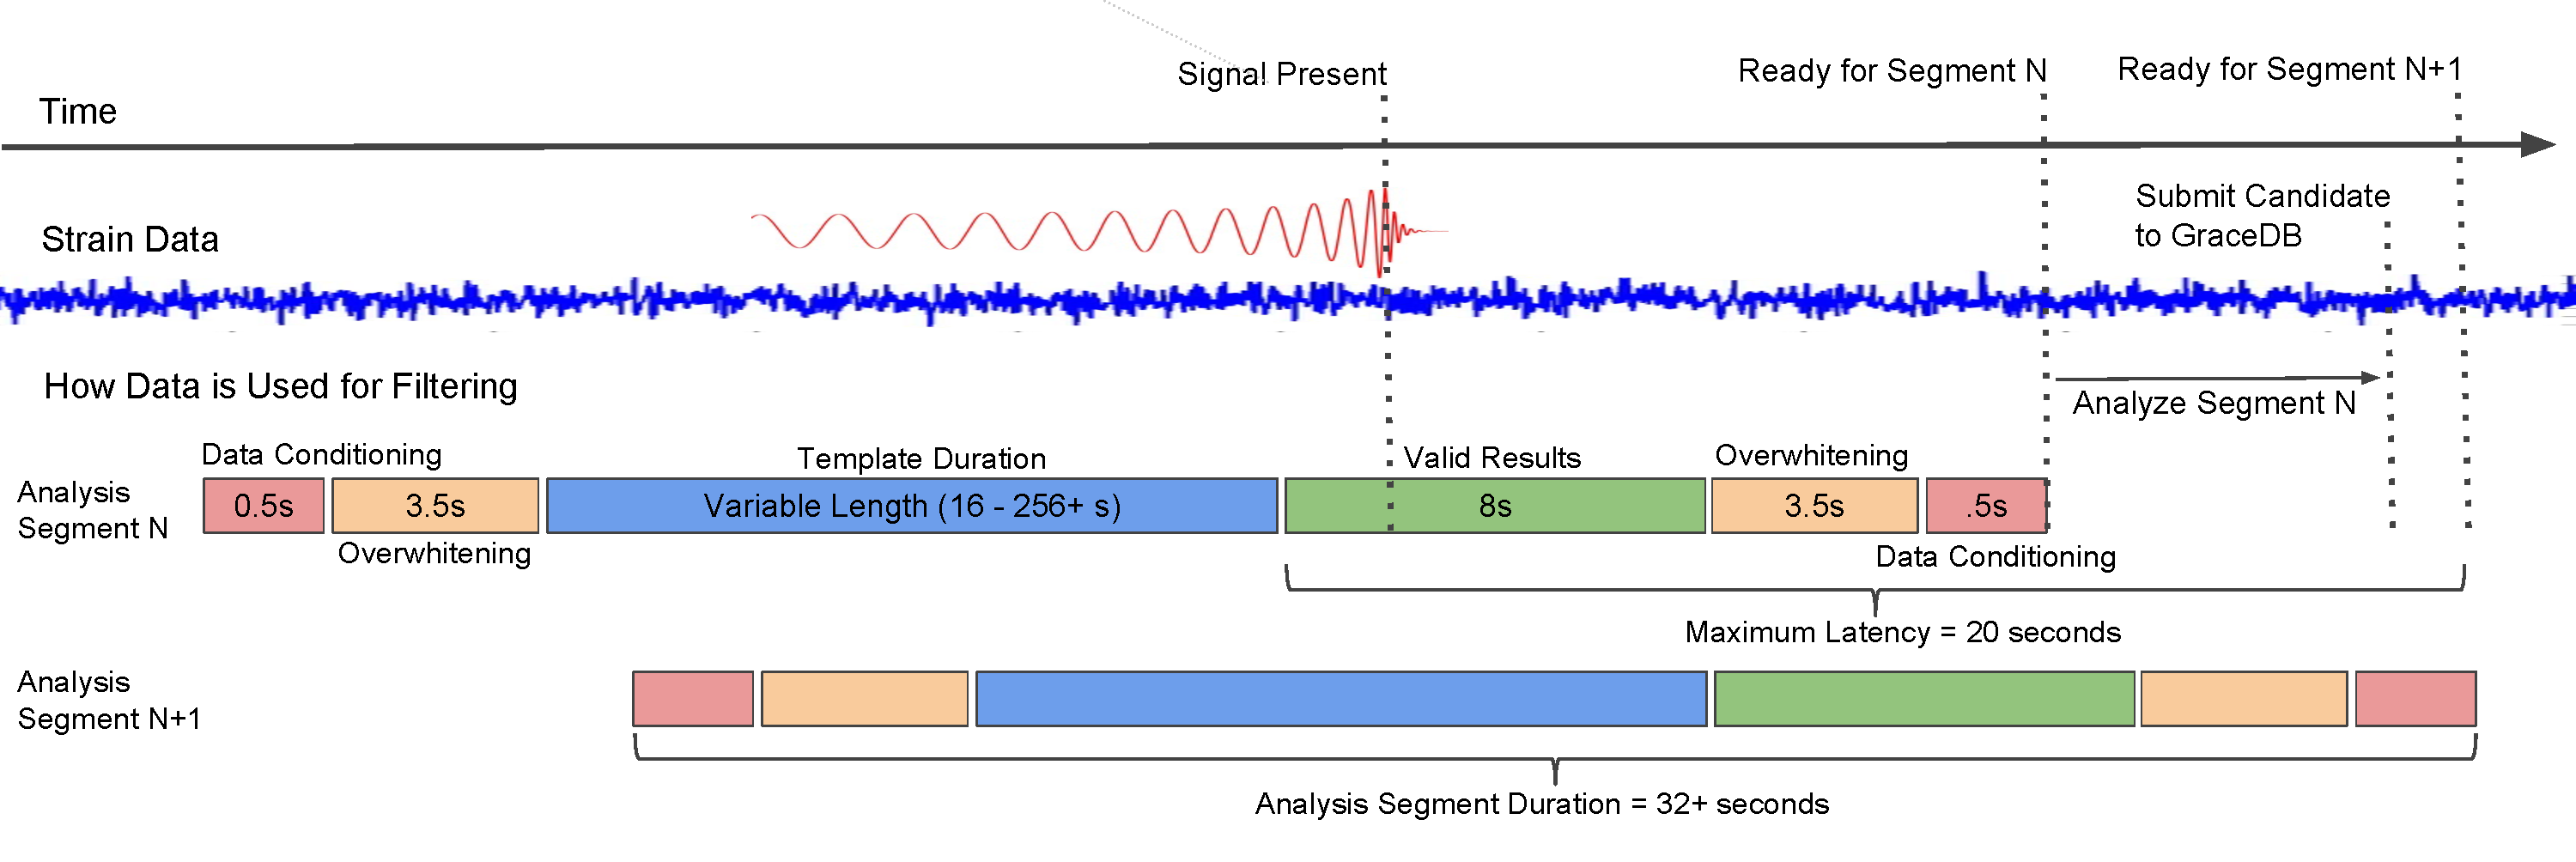
\includegraphics[width=1.0\linewidth]{images/2_searches/live_latency_diagram.pdf}
    \caption{Caption}
    \label{2:fig:live_latency_diagram}
\end{figure}
%
The PyCBC Live search aims to detect all gravitational waves in real time. This is a feat of software engineering to obtain the gravitational wave data, perform the matched filtering of hundreds of thousands of templates, perform signal consistency tests and output an approximate sky map within tens of seconds of the merger of the gravitational wave passing through the detectors.

The live search is distributed over 151 computing nodes and these are all connected through a message passing interface which tracks the individual search nodes. The main ranked node will receive messages from each of these nodes and distribute information and jobs to all the nodes. For example, when a node running a matched filter on H1 data finds a trigger and a node running a matched filter on L1 data finds a trigger, these triggers are sent back to the rank 0 node which then assigns another node to perform the coincidence tests as part of the ranking statistic to determine if this trigger was a real gravitational wave event.

The template bank of 730 thousand template distributed throughout the nodes and pre-generated in memory so the matched filters do not have to rely on generating the templates every time new data arrives. The template bank is shuffled into a random order so that the distribution of `long' and `short' templates is randomly distributed throughout the nodes. If a single node has all the long templates it will take longer to perform the matched filters than the nodes with the short templates and this can introduce lagging effects if the search is being held up by a single node.

The live search holds a continuous buffer of data where the newest eight seconds of data are added to the front and push the oldest eight seconds of data out of the buffer. The data is then matched filtered with the template bank and each node reports on the triggers that have been found. The hope with the search is that all of this processing can happen before the next eight seconds of data arrives at the detector. (PLOT: PYCBC LIVE LAG PLOT DIAGRAM THING)

\subsection{\label{2:sec:snr-optimization}SNR Optimization}

We upload potential detections of gravitational wave events to a central public database called GraceDB. These events are then used by astronomers to observe potential electromagnetic counterparts. We want to report the best information we can and produce the most accurate sky map. Increasing the SNR of the event is an easy way to improve this, having a better matching template to the signal will do this. (REWRITE).

The SNR optimization module of PyCBC Live takes a gravitational wave event and uses optimization functions to rapidly optimize the gravitational wave parameters to retrieve small fractions of improvement to the SNR. The original SNR of the event is limited by the template bank placement and the SNR optimizer allows a much finer exploration of the local parameter space to the best found template in the template bank. (ADD PLOT SHOWING TEMPLATE BANK WITH TEMPLATES NEARBY THE ACTUAL PARAMETER VALUES AND SNR IMPROVEMENT).

\subsection{\label{2:sec:live-ranking-statistic}Ranking Statistic}

The PyCBC Live ranking statistic run in the third observing run and the first half of the fourth observing run was very simple, only taking into account the Allen chisq, sine-gaussian chisq and phasetd. These are basic signal consistency tests for single detector checks, re-ranking the snr depending on how the morphology of the snr evolves over the signal. In coincidence the ranking statistic only looks for phase and template consistency for the two triggers and a time coincidence so that both detector triggers fall in light time travel time.



% Removed from pycbclive.tex
This chapter details the changes made to the PyCBC Live ranking statistic to improve on the original ranking statistic used in the third and fourth observing runs and detailed in~\ref{2:sec:live-ranking-statistic}. The two additions that were made to the ranking statistic were the inclusion of PSD variation, to track the non-stationary of the detector noise, and adding template fits to the statistic to weigh triggers based on their previously measured SNR distribution.

In this chapter we introduce the PyCBC Live search for CBC signals and the improvements made to the PyCBC Live search's ranking statistic to improve the sensitivity of the search and the confidence of our gravitational wave detections. The PyCBC Live search has been operational since the 2018~\cite{PyCBC_Live:2018} and has been in constant operation since, contributing to the 2nd, 3rd and 4th observing runs and detecting over 200 gravitational wave events. The PyCBC Live search processes gravitational wave detector data using techniques described in section~REMOVED however, there are a number of optimizations and new techniques used to enable to low-latency rapid detection of gravitational wave events in close to real time.

PyCBC Live uses a ranking statistic post-detection of a gravitational wave event candidate which provides a numerical confidence in the event being real. This number is referred to as the `False Alarm rate' (FAR) and is measured in units of events per unit time (typically per year or Hertz). The inverse of the false alarm rate (IFAR) is commonly used and is typically measured in units of years. The false alarm rate tells us how often a candidate event would be observed due to random noise in the absence of a real astrophysical signal. IFAR can be thought of as the expected time interval between random noise events that could produce a signal resembling the observed candidate event. A higher IFAR indicates a longer expected waiting time between false alarms.

The LVK places a limit on the IFAR of a signal before it can be determined to be real. The limit has to be placed to balance the sensitivity of a search and the purity of a gravitational wave catalogue. As a quick example, if the IFAR limit is set to 1 year. Then one might expect to see one event per year in the catalog purely due to noise.

We begin this chapter by detailing the components that make up the ranking statistic and then the new components of the improved ranking statistic and how these are derived and used.

\section{\label{2:sec:current-detections}Gravitational-Wave Observations to date}
